We need a small intro explaining the purpose of this chapter, like the main goal is to prove the Vinagradov mean value theorem. 
For that we prove the more general result about decoupling and then use it in the context of exponential sums.\\

Introduce the definition. Maybe motivate why this partion is natural in the case of curves. It has to obey nicely an affine rescaling (Guth notes). \\

Move onto the the bilinear reduction. Calculations for the change of variables.  Whitney (tenho de fazer boneco). \\

Introduce billinear assymetric, mention that the BDG object is more complicated. Talk about the tranversality is captured by the assymetric constantes.\\

Change the proof of lower degree decoupling (call it Pranik-Seeger iteration because this is how we extend the result to the circle for instance). Show how to prove the dilation.\\ 

Key lemma, show to get the C. Use the picture to explain. Use the reduction, where one box uses the center. Refer back to the averaging result showed in parabola. (Invoke appendix lemmas). 

Do the final steps for the iteration.\\

(one needs the linear algebra result).
\newpage
\section{Intro stuff - geometry and definitions}
To generalize the work done in Chapter 2, we need to establish which neighborhood of the curve we are choosing and how to partition it in \(\mathbb{R}^k\). For curves, the appropriate scale to consider is \(\delta^k\). This choice essentially arises from the need to obtain the correct scale when reframing the problem under a change of coordinates [Guth, Lecture18].


Let $\Gamma:[0,1] \rightarrow \mathbb{R}^{k}$ be the moment curve in $\mathbb{R}^{k}$, parametrized by 
$$
\Gamma(\xi):=\left(\xi, \xi^{2}, \ldots, \xi^{k}\right).
$$
Let $\theta$ be a $\delta^k$-arc of the moment curve, i.e, is $\Gamma([a,a+\delta^k])$ for some $a$. Then by Taylor expansion, 


$$\Gamma(t)=\Gamma\left(c_a\right)+\Gamma^{\prime}\left(c_a\right) \Delta t+\frac{1}{2} \Gamma^{\prime \prime}\left(c_a\right) \Delta t^{2}+\cdots+\frac{1}{k!} \Gamma^{(k)}\left(c_a\right) \Delta t^{k}$$. 

Observing that  $\Delta t^j$ as size proportional to $\delta^j$ and that $\Gamma^{\prime}\left(c_a\right), \Gamma^{\prime \prime}\left(c_a\right), \cdots, \Gamma^{(k)}\left(c_a\right)$ are linear independent the smallest box that can contain $\theta $ has dimensions $\delta \times \delta^2\times \cdots \delta^k$. 

For $\delta \in(0,1)$, let $\mathcal{P}(\delta)$ denote the partition of the interval $[0,1]$ into dyadic intervals with length $2^{-\left\lceil\log _{2} \delta^{-1}\right\rceil}$. For a dyadic interval $J$, let $\mathcal{U}_{J}$ be the parallelepiped of dimensions $|J|^{1} \times|J|^{2} \times \cdots \times|J|^{k}$ whose center is $\Gamma\left(c_{J}\right)$ and sides are parallel to $\partial^{1} \Gamma\left(c_{J}\right), \partial^{2} \Gamma\left(c_{J}\right), \ldots$, $\partial^{k} \Gamma\left(c_{J}\right)$, where $c_{J}$ is the center of $J$. In a similar way we make the following notation simplifications, write $p_{k}:=k(k+1)$ for the critical exponent, and $\|\cdot\|_{p}:=\|\cdot\|_{L^{p}\left(\mathbb{R}^{k}\right)}$.

\begin{defn}\label{defn:gen_moment}
For $\delta \in(0,1)$, the $\ell^{2} L^{p_{k}}$ decoupling constant $\Dec_{k}(\delta)$ for the moment curve in $\R^k$ is the smallest number for which the inequality

\begin{equation*}
\left\|\sum_{J \in \mathcal{P}(\delta)} f_{J}\right\|_{p_{k}} \leqslant \mathcal{D}_{k}(\delta)\left(\sum_{J \in \mathcal{P}(\delta)}\left\|f_{J}\right\|_{p_{k}}^{2}\right)^{1 / 2} 
\end{equation*}

holds for any tuple of functions $\left(f_{J}\right)_{J \in \mathcal{P}(\delta)}$ with $\supp\widehat{f_{J}} \subseteq \mathcal{U}_{J}$ for all $J$.
\end{defn}
\begin{thm}\label{thm:main_moment}
 For every $k \in \mathbb{N}$ and every $\epsilon>0$, there exists a finite constant $C_{k, \epsilon}$ such that
\begin{equation*}
\mathcal{D}_{k}(\delta) \leqslant C_{k, \epsilon} \delta^{-\epsilon}, \text { for every } \delta \in(0,1)
\end{equation*}
\end{thm}

By choosing this geometry for the frequency space we can get the analogous property of parabolic rescaling (citar chapter 2).
Recall, that for $I=[a,a+h]$,

$$
\Gamma(a+th)= \Gamma(a)+ \sum_{j=1}^{k}\frac{\partial^{j}\Gamma(a)}{j!}(ht)^j.
$$
Let
\[
DJ_I = \left[ \begin{array}{c|c|c|c}
\partial^1 \Gamma(a) & \partial^2 \Gamma(a) & \cdots & \partial^k \Gamma(a)
\end{array} \right]
\]

and

\[
D_h = \mathrm{diag}\left(\frac{h}{1!}, \frac{h^2}{2!}, \cdots, \frac{h^k}{k!}\right).
\] and define the following map $A_I:\xi \xrightarrow{} \Gamma(a)+DJ_I D_h \xi$, then $A_I\Gamma(t)=\Gamma(a+th)$, for all $t\in \R$, i.e we can map a subset of the curve to the whole curve. 

It follows that, for dyadic intervals $I, J$ with $J \subset I \subset[0,1]$, we have

$$
A_{I}^{-1} \mathcal{U}_{J}=\mathcal{U}_{J_{I}}
$$

where $J_{I}:=h^{-1}(J-a)$ if $I=[a, a+h]$. 
To see why this is true, recall that
$$
\calU_{I}= \left\{ \Gamma(C_I)+\sum_{l=1}^{k} r_l \frac{\partial^{l}\Gamma(a)}{l!}(ht)^l\, |r_l|\sim\text{,}\, |J|^l\right\}
$$
and take $\xi\in \calU_{J}$ and with $t_J$ such that $C_J= a+t_J h$.
$$
\xi = \Gamma(a+t_J h)+\sum_{l=1}^{k} r_l \frac{\partial^{l}\Gamma(a+t_J h)}{l!}(ht)^l,
$$
then by applying $A^{-1}_I$ 
$$
A^{-1}_I\xi = \Gamma(t_J)+\sum_{l=1}^{k} r_l\,h^{-l} \frac{\partial^{l}\Gamma(t_J)}{l!}.
$$
which givesd the desired conclusion.
\subsection{Billinear approach}
As discussed in (citar subsection), in decoupling theory, introducing an appropriate multilinear object can significantly facilitate the analysis. Selecting the right object is crucial and involves a nuanced understanding of the problem. For instance, in $k$ dimensions, one might consider using a $k$-multilinear object. However, this is not quite the right degree as was demonstrated by Bourgain, Guth, and Demeter [BGD16, section 6], in the first harmonic analysis-based proof of Vinogradov's mean value theorem where they required a $k!$-multilinear object.   

In this approach, we instead use $k$ bilinear objects, each contributing information about the decoupling constant at different dimensions. These objects are carefully designed to facilitate the iteration procedure and are closely linked to Wooley's method of efficient congruencing, which provided the second proof for Vinogradov's mean value theorem. For further explanations on the connections between these two methods, see [LillianPierce].


For the sake of clarity, we first present a bilinear reduction using a symmetric object. We then demonstrate how this reduction relates to the primary objects of study, establishing a connection between the bilinear approach and the overarching framework.

\begin{defn}
    For $\delta \in(0,1 / 4)$, the symmetric bilinear decoupling constant $\mathcal{B}(\delta)$ for the moment curve $\Gamma$ in $\mathbb{R}^{k}$ is the smallest constant such that, for any pair of intervals $I, I^{\prime} \in$ $\mathcal{P}(1 / 4)$ with $\operatorname{dist}\left(I, I^{\prime}\right) \geqslant 1 / 4$ and any tuple of functions $\left(f_{J}\right)_{J \in \mathcal{P}(I, \delta) \cup \mathcal{P}\left(I^{\prime}, \delta\right)}$ with supp $\widehat{f_{J}} \subseteq$ $\mathcal{U}_{J}$ for all $J$, the following inequality holds:

\begin{equation*}
\int_{\mathbb{R}^{k}}\left|f_{I}\right|^{p_{k} / 2}\left|f_{I^{\prime}}\right|^{p_{k} / 2} \leqslant \mathcal{B}(\delta)^{p_{k}}\left[\sum_{J \in \mathcal{P}(I, \delta)}\left\|f_{J}\right\|_{p_{k}}^{2}\right]^{p_{k} / 4}\left[\sum_{J^{\prime} \in \mathcal{P}\left(I^{\prime}, \delta\right)}\left\|f_{J^{\prime}}\right\|_{p_{k}}^{2}\right]^{p_{k} / 4} 
\end{equation*}

\end{defn}

\begin{lem}[Bilinear reduction]\label{lem:bil_redu}
If $\delta=2^{-N}$, then

\begin{equation*}
\mathcal{D}_{k}(\delta) \lesssim\left(1+\sum_{n=2}^{N} \mathcal{B}\left(2^{-N+n-2}\right)^{2}\right)^{1 / 2}.
\end{equation*}
\end{lem}

The proof essentially relies of affine rescaling and a Whitney decomposition of $[0,1]^2$. 

\begin{rmk}
    We could also have used this decompositon for the parabola case.
\end{rmk}
\begin{figure}[h!]
    \centering
    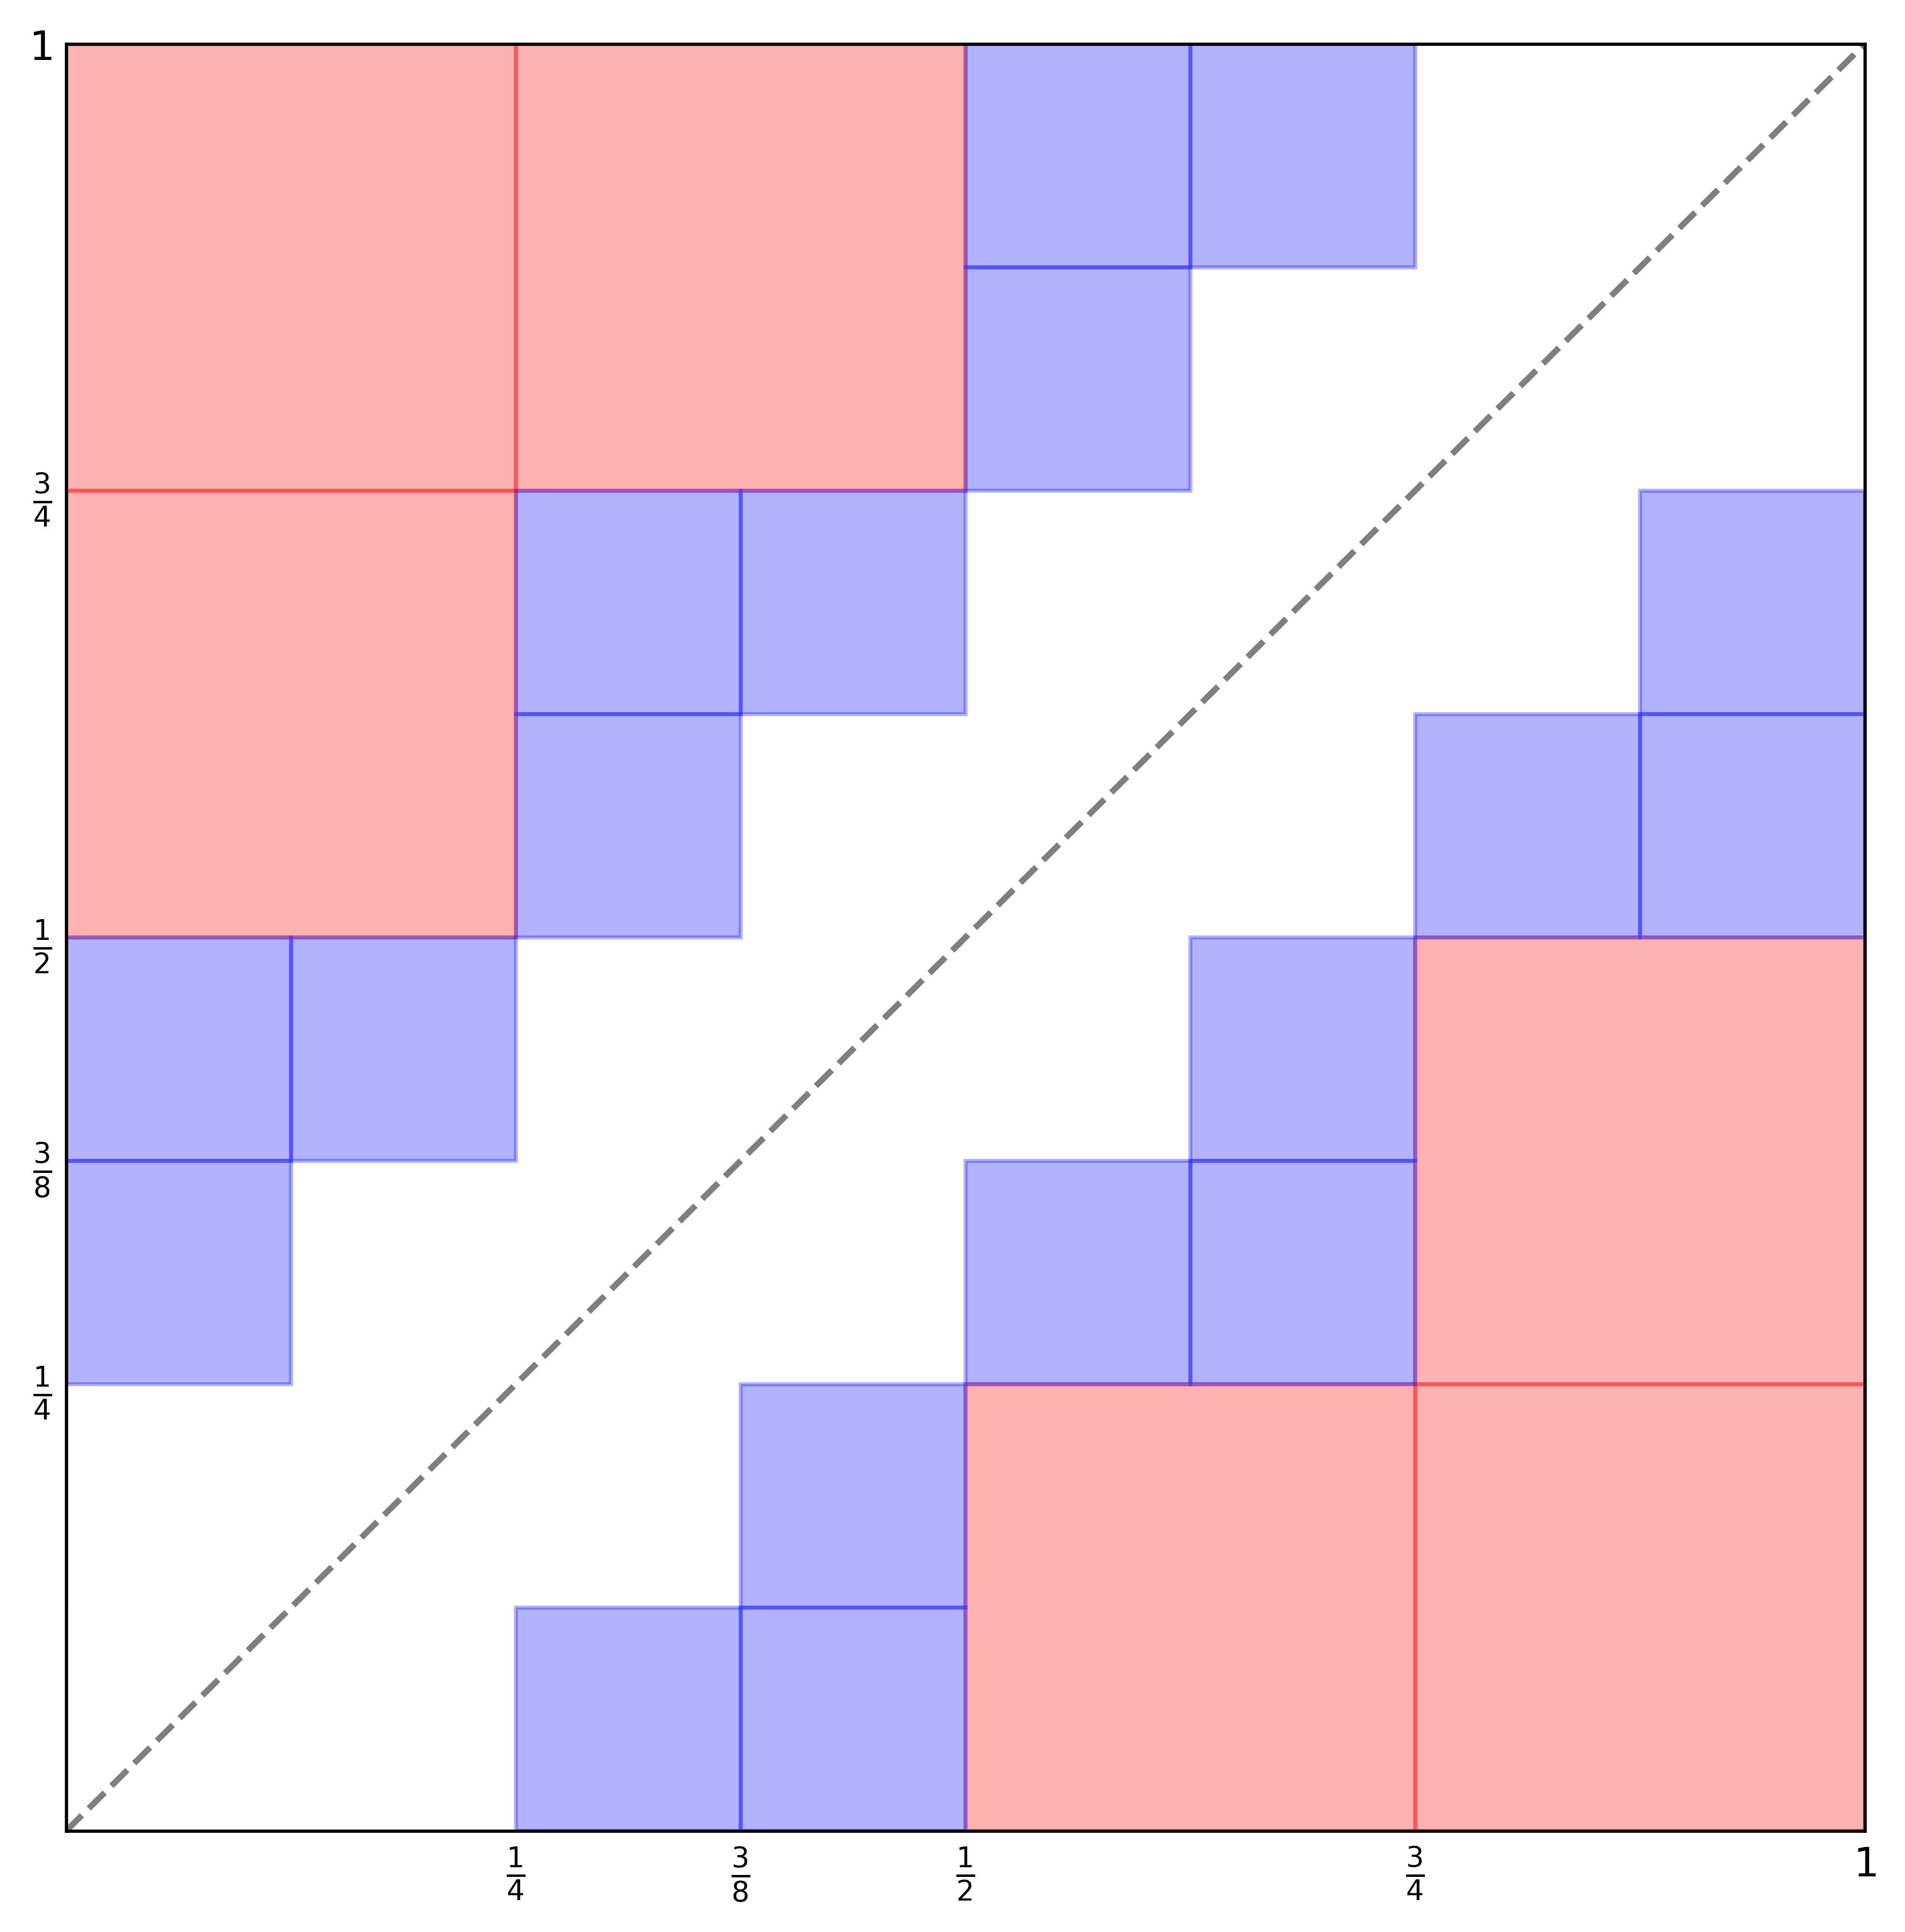
\includegraphics[scale=0.5]{/home/dnf/Downloads/Thesis/Chapters/General curve/whitney_decomp.png}
    \caption{Whitney decompostion}
    \label{fig:whitney}
\end{figure}


\begin{lem}
 Let $I \in \mathcal{P}\left(2^{-n}\right)$ for some integer $n \geqslant 0$. For any $\delta \in\left(0,2^{-n}\right)$ and any tuple of functions $\left(f_{J}\right)_{J \in \mathcal{P}(I, \delta)}$ with $\operatorname{supp} \widehat{f_{J}} \subseteq \mathcal{U}_{J}$ for all $J$, the following inequality holds:


\begin{equation*}
\left\|f_{I}\right\|_{p_{k}} \leqslant \mathcal{D}_{k}\left(2^{n} \delta\right)\left(\sum_{J \in \mathcal{P}(I, \delta)}\left\|f_{J}\right\|_{p_{k}}^{2}\right)^{1 / 2} 
\end{equation*}

Let $I, I^{\prime} \in \mathcal{P}\left(2^{-n}\right)$ for some integer $n \geqslant 2$ with $2^{n} \operatorname{dist}\left(I, I^{\prime}\right) \in\{1,2\}$. For any $\delta \in\left(0,2^{-n}\right)$ and any tuple of functions $\left(f_{J}\right)_{J \in \mathcal{P}(I, \delta) \cup \mathcal{P}\left(I^{\prime}, \delta\right)}$ with $\operatorname{supp} \widehat{f_{J}} \subseteq \mathcal{U}_{J}$ for all $J$, the following inequality holds:


\begin{equation*}
\int_{\mathbb{R}^{k}}\left|f_{I}\right|^{p_{k} / 2}\left|f_{I^{\prime}}\right|^{p_{k} / 2} \leqslant \mathcal{B}\left(2^{n-2} \delta\right)^{p_{k}}\left[\sum_{J \in \mathcal{P}(I, \delta)}\left\|f_{J}\right\|_{p_{k}}^{2}\right]^{p_{k} / 4}\left[\sum_{J^{\prime} \in \mathcal{P}\left(I^{\prime}, \delta\right)}\left\|f_{J^{\prime}}\right\|_{p_{k}}^{2}\right]^{p_{k} / 4} 
\end{equation*}
\end{lem}
\begin{proof}
    See where to prove this. Here or in chapter 2. (It's the same thing)
\end{proof}
\begin{proof}[Proof of Lemma \ref{lem:bil_redu}]
Suppose that $\delta=2^{-N}$. Set $\mathcal{W}_{1}:=\varnothing$. For integers $n \geqslant 2$, define iteratively

$$
\mathcal{W}_{n}:=\left\{\left(I_{1}, I_{2}\right) \in \mathcal{P}\left(2^{-n}\right) \mid 2^{n} \operatorname{dist}\left(I_{1}, I_{2}\right) \in\{1,2\} \text { and } I_{1} \times I_{2} \notin \bigcup_{\left(I_{1}^{\prime}, I_{2}^{\prime}\right) \in \mathcal{W}_{n-1}} I_{1}^{\prime} \times I_{2}^{\prime}\right\}
$$

For each $n\geq2$, $\mathcal{W}_n$ contains the squared of side length $2^{-n}$ present in the decomposition. Since we are only interested in information about the norms up to scale $2^{-N}$ we need to stop the decomposition at this stage. To turn this into partition of $[0,1]^2$ had the diagonal pieces at scale $2^{-N}$,


$$
\widetilde{\mathcal{W}}_{N}:=\left\{\left(I_{1}, I_{2}\right) \in \mathcal{P}\left(2^{-N}\right) \mid \operatorname{dist}\left(I_{1}, I_{2}\right)=0\right\}.
$$

Then, 

$$
\mathcal{W}^{N}:=\bigcup_{n=2}^{N} \mathcal{W}_{n} \cup \widetilde{\mathcal{W}}_{N}
$$

form an essentially disjoint (up to boundaries) covering of $[0,1]^{2}$. Let $\left(f_{J}\right)_{J \in \mathcal{P}(\delta)}$ be as in Definition \ref{defn:gen_moment} for $\mathcal{D}_{k}(\delta)$. Then


\begin{align*}
\left\|\sum_{J \in \mathcal{P}(\delta)} f_{J}\right\|_{p_{k}} & =\left\|\sum_{\left(I, I^{\prime}\right) \in \mathcal{W}^{N}} f_{I} \overline{f_{I^{\prime}}}\right\|_{p_{k} / 2}^{1 / 2} \leqslant\left(\sum_{\left(I, I^{\prime}\right) \in \mathcal{W}^{N}}\left\|f_{I} \overline{f_{I^{\prime}}}\right\|_{p_{k} / 2}\right)^{1 / 2} \\
& \leqslant\left(\sum_{\left(I, I^{\prime}\right) \in \widetilde{\mathcal{W}}_{N}}\left\|f_{I}\right\|_{p_{k}}\left\|f_{I^{\prime}}\right\|_{p_{k}}+\sum_{n=2}^{N} \sum_{\left(I, I^{\prime}\right) \in \mathcal{W}_{n}}\left\|f_{I} \overline{f_{I^{\prime}}}\right\|_{p_{k} / 2}\right)^{1 / 2}
\end{align*}

We estimate the first term by

$$
\sum_{I, I^{\prime} \in  \widetilde{\mathcal{W}}_{N}}\left(\left\|f_{I}\right\|_{p_{k}}^{2}+\left\|f_{I^{\prime}}\right\|_{p_{k}}^{2}\right) \leqslant 6 \sum_{I \in \mathcal{P}\left(2^{-N}\right)}\left\|f_{I}\right\|_{p_{k}}^{2}
$$

since each $I$ appears at most 6 times in the pairs $\widetilde{\mathcal{W}}_{N}$. In the second term, by affine rescaling (), for every $\left(I, I^{\prime}\right) \in \mathcal{W}_{n}$, we have

\[
\begin{aligned}
\left\|f_{I} \overline{f_{I^{\prime}}}\right\|_{p_{k} / 2} & \lesssim \mathcal{B}\left(2^{-N+n-2}\right)^{2} \left( \ell_{J \in \mathcal{P}(I, 2^{-N})}^{2} \left\|f_{J}\right\|_{p_{k}} \right) \left( \ell_{J^{\prime} \in \mathcal{P}(I^{\prime}, 2^{-N})}^{2} \left\|f_{J^{\prime}}\right\|_{p_{k}} \right) \\
& \lesssim \mathcal{B}\left(2^{-N+n-2}\right)^{2} \left(\left( \ell_{J \in \mathcal{P}(I, 2^{-N})}^{2} \left\|f_{J}\right\|_{p_{k}} \right)^{2} + \left( \ell_{J^{\prime} \in \mathcal{P}(I^{\prime}, 2^{-N})}^{2} \left\|f_{J^{\prime}}\right\|_{p_{k}} \right)^{2} \right)
\end{aligned}
\]


Since each $I \in \mathcal{P}\left(2^{-n}\right)$ appears at most 8 times in $\mathcal{W}_{n}$, it follows that

$$
\sum_{\left(I, I^{\prime}\right) \in \mathcal{W}_{n}}\left\|f_{I} \overline{f_{I^{\prime}}}\right\|_{p_{k} / 2} \lesssim \mathcal{B}\left(2^{-N+n-2}\right)^{2}\left( \ell_{J \in \mathcal{P}(2^{-N})}^{2} \left\|f_{J}\right\|_{p_{k}} \right)
$$

Inserting these bounds in (2.5), we obtain the desired estimate.
\end{proof}

\subsection{Main object}
In this subsection we develop the essential ingredients for the main object of study. We start by introducing some standard... 

Introduce the $k$ bilinear objects and essencially reproduce the averaging argument done in (chapter 2). That approach heavly relies of the uncertaintly principle, so we need to formalize it in the context of this problem.
For a dyadic interval $I$, let $\freqU_{I}$ denote the parallelepiped centered at the origin dual to $\calU_{I}$, that is,

$$
\freqU_{I}:=\left\{\left.x \in \mathbb{R}^{k}:|\left\langle x, \partial^{i} \Gamma\left(c_{I}\right)\right\rangle|\leqslant| I\right|^{i}, 1 \leqslant i \leqslant k\right\}.
$$



Here, \( A \) represents a dimensional constant with specific requirements: \( A > k \) and \( A \geqslant \frac{k(k+1)}{2} \). One can interpret \( \phi_{I} \) as a smoother version of the indicator function \( |\freqU_{I}|^{-1}\mathrm{1}_{\freqU_{I}} \), remaining constant inside \( \freqU_{I} \) and decaying rapidly outside. Lemmas A.1 and A.2 provide further insights into why these conditions are necessary for the decay behavior of \( \phi_{I} \). Furthermore, one can see that the $L^1$ norm is independent of the chosen interval.\\

Let \( M_{I} \) and \( \phi \) be defined in the following way:

\begin{equation}\label{eq:change_box}
M_{I} = \left[ \begin{array}{c|c|c|c}
\partial^1 \Gamma(c_{I}) & \partial^2 \Gamma(c_{I}) & \cdots & \partial^k \Gamma(c_{I})
\end{array} \right]
\end{equation}

and 

\begin{equation}\label{eq:function_change_box}
\phi_{\delta}(x)= \delta^{k(k+1)/2} \max \{1, \delta |x_1|, \cdots, \delta^{k} |x_k|\}^{-A}.
\end{equation}

Observing that \(\langle (M_{I}^{-1})^{\top} x, \partial^i \Gamma \rangle = \langle x, M_{I}^{-1} \partial^i \Gamma \rangle = \langle x, e_i \rangle\), the following can be seen as an expression invariant under the choice of interval after an elementary change of variables:

\[
\int_{\R^k} \phi_{I}(x)\, dx = \int_{\R^k} \phi_{I}((M^{-1})^{\top} x)\, dx = \int_{\R^k} \phi_{\delta}(x)\, dx.
\]

\begin{lem}[Uncertaintly principle]\label{lem:uncer.prin.}
    For $p \in[1, \infty)$ and $J \subset[0,1]$, we have

$$
\left|g_{J}\right|^{p} \lesssim_{p}\left|g_{J}\right|^{p} * \phi_{J}
$$

for every $g_{J}$ with $\operatorname{supp} \widehat{g_{J}} \subseteq C \mathcal{U}_{J}$.

\end{lem}
\begin{proof}
Let $\psi$ be a Schwartz function adapted to $\mathcal{U}_{J}^{\circ}$ such that $\hat{\psi} \equiv 1$ on $C \mathcal{U}_{J}$ and $\int|\psi| \approx 1$. Then $g_{J}=g_{J} * \psi$, so


\begin{align*}
\left|g_{J}\right|^{p}(x) & \leqslant\left(\int\left|g_{J}(x-z)\right|^{p}|\psi(z)| \mathrm{d} z\right)\left(\int|\psi(z)| \mathrm{d} z\right)^{p / p^{\prime}}\\
& \lesssim\left(\left|g_{J}\right|^{p} *|\psi|\right)(x) \lesssim\left(\left|g_{J}\right|^{p} * \phi_{J}\right)(x)
\end{align*}

\end{proof}
As a mater of fact, under the support hypothesis of (\ref{lem:uncer.prin.}) the function $\left|g_{J}\right|^{p} * \phi_{J}$ rigorously satisfies the heuristic of being essentially constant on translates of the dual box. Define
$$\mathcal{U}_{\delta} =\{x\in \R^k\text{: } \forall i\text{, } |x_i|\leq \delta^{i} \}, $$ then $x\in \mathcal{U}_{\delta}$ if and only if $(M_{J})^{\top}x \in \freqU_{J}$.
Take $x \in \mathcal{U}_{\delta}$ and proceed as above to obtain 
$$\left|g_{J}\right|^{p} * \phi_{J}((M_{J}^{-1})^{\top}x_{1}) = \int_{\R^k} |g_{J}|^{p}(y)\phi_{J}((M_{J}^{-1})^{\top}x_{1}-y)dy \sim 
\int_{\R^k} |g_{J}|^{p}((M_{J}^{-1})^{\top}y)\phi_{J}((M_{J}^{-1})^{\top}(x_{1}-y))dy. 
$$
By using an analogous formula to \ref{eq:function_change_box}, one can see that for $x_1$ $x_2$ $\in \mathcal{U}_\delta$, $$\left|g_{J}\right|^{p} * \phi_{J}((M_{J}^{-1})^{\top}x_{1}) \sim \left|g_{J}\right|^{p} * \phi_{J}((M_{J}^{-1})^{\top}x_{2}),$$ with absolute constant independent of the size of $J$.

Motivated by this formulation of the uncertainly principle we now define the main objects of study in the following way:

\begin{defn}\label{def:assymetric}
     For $l \in\{0, \ldots, k-1\}, a, b \in[0,1]$ and $\delta \in(0,1)$, 
     the (asymmetric) bilinear decoupling constant $\mathcal{B}_{l, a, b}(\delta)$ for the moment curve 
     $\Gamma$ in $\hat{\mathbb{R}}^{k}$ is the smallest constant such that, 
     for all pairs of intervals $I \in \mathcal{P}\left(\delta^{a}\right), I^{\prime} \in \mathcal{P}\left(\delta^{b}\right)$
      with $\operatorname{dist}\left(I, I^{\prime}\right) \geqslant 1 / 4$ and all tuples of functions 
      $\left(f_{J}\right)_{J \in \mathcal{P}(I, \delta) \cup \mathcal{P}\left(I^{\prime}, \delta\right)}$
       with supp $\widehat{f_{J}} \subseteq \mathcal{U}_{J}$ for all $J$, the following inequality holds:


\begin{align*}
& \int_{\mathbb{R}^{k}}\left(\left|f_{I}\right|^{p_{l}} * \phi_{I}\right)\left(\left|f_{I^{\prime}}\right|^{p_{k}-p_{l}} * \phi_{I^{\prime}}\right) \\
& \leqslant \mathcal{B}_{l, a, b}(\delta)^{p_{k}}\left[\sum_{J \in \mathcal{P}(I, \delta)}\left\|f_{J}\right\|_{p_{k}}^{2}\right]^{p_{l} / 2}\left[\sum_{J^{\prime} \in \mathcal{P}\left(I^{\prime}, \delta\right)}\left\|f_{J^{\prime}}\right\|_{p_{k}}^{2}\right]^{\left(p_{k}-p_{l}\right) / 2} 
\end{align*}

\end{defn}

\begin{rmk}
     In the case $l=0$, the bilinear decoupling constant $\mathcal{B}_{0, a, b}(\delta)$  does not depend on $a$, by using affine rescaling (citar affine rescaling), we have


\begin{equation*}
\mathcal{B}_{0, a, b}(\delta) \sim \mathcal{D}_{k}\left(\delta^{1-b}\right).
\end{equation*}

\end{rmk}

\begin{lem}\label{lem:sym.to.asym.}
For every $l \in\{0, \ldots, k-1\}, a, b \in[0,1]$ and $\delta \in(0,1 / 4)$, we have

\begin{equation*}
\mathcal{B}(\delta) \lesssim \delta^{-a p_{l} / p_{k}} \delta^{-b\left(p_{k}-p_{l}\right) / p_{k}} \mathcal{B}_{l, a, b}(\delta) \tag{3.4}
\end{equation*}

\end{lem}

\begin{proof}
    Let $I, I^{\prime} \in \mathcal{P}(1 / 4)$ with $\operatorname{dist}\left(I, I^{\prime}\right) \geqslant 1 / 4$. Let $\left(f_{K}\right)_{K \in \mathcal{P}(I, \delta) \cup \mathcal{P}\left(I^{\prime}, \delta\right)}$ be a tuple of functions with supp $\widehat{f_{K}} \subseteq \mathcal{U}_{K}$ for all $K$. By Hölder's inequality, we have


\begin{equation*}
\int_{\mathbb{R}^{k}}\left|f_{I}\right|^{p_{k} / 2}\left|f_{I^{\prime}}\right|^{p_{k} / 2} \leqslant\left(\int_{\mathbb{R}^{k}}\left|f_{I}\right|^{p_{l}}\left|f_{I^{\prime}}\right|^{p_{k}-p_{l}}\right)^{1 / 2}\left(\int_{\mathbb{R}^{k}}\left|f_{I}\right|^{p_{k}-p_{l}}\left|f_{I^{\prime}}\right|^{p_{l}}\right)^{1 / 2} \tag{3.5}
\end{equation*}


By symmetry, it suffices to estimate the first bracket. Assume that $l \neq 0$; the case $l-0$ is similar, but easier, since the term with power $p_{l}$ disappears. We have

$$
\begin{aligned}
\int_{\mathbb{R}^{k}}\left|f_{I}\right|^{p_{l}}\left|f_{I^{\prime}}\right|^{p_{k}-p_{l}} & \leqslant \int_{\mathbb{R}^{k}}\left(\sum_{J \in \mathcal{P}\left(I, \delta^{a}\right)}\left|f_{J}\right|\right)^{p_{l}}\left(\sum_{J^{\prime} \in \mathcal{P}\left(I^{\prime}, \delta^{b}\right)}\left|f_{J^{\prime}}\right|\right)^{p_{k}-p_{l}} \\
& \leqslant\left|\mathcal{P}\left(I, \delta^{a}\right)\right|^{p_{l}-1}\left|\mathcal{P}\left(I^{\prime}, \delta^{b}\right)\right|^{p_{k}-p_{l}-1} \sum_{J \in \mathcal{P}\left(I, \delta^{a}\right)} \sum_{J^{\prime} \in \mathcal{P}\left(I^{\prime}, \delta^{b}\right)} \int_{\mathbb{R}^{k}}\left|f_{J}\right|^{p_{l}}\left|f_{J^{\prime}}\right|^{p_{k}-p_{l}}
\end{aligned}
$$

By Lemma 3.3 and Definition 3.1, we have

$$
\begin{aligned}
\int_{\mathbb{R}^{k}}\left|f_{J}\right|^{p_{l}}\left|f_{J^{\prime}}\right|^{p_{k}-p_{l}} & \lesssim \int_{\mathbb{R}^{k}}\left(\left|f_{J}\right|^{p_{l}} * \phi_{J}\right)\left(\left|f_{J^{\prime}}\right|^{p_{k}-p_{l}} * \phi_{J^{\prime}}\right) \\
& \leqslant \mathcal{B}_{l, a, b}(\delta)^{p_{k}}\left[\ell_{K \in \mathcal{P}(J, \delta}^{2}\left\|f_{K}\right\|_{p_{k}}\right]^{p_{l}}\left[\ell_{K^{\prime} \in \mathcal{P}\left(J^{\prime}, \delta\right)}^{2}\left\|f_{K^{\prime}}\right\|_{p_{k}}\right]^{p_{k}-p_{l}}
\end{aligned}
$$

Inserting this into the previous display, and using $\ell^{2} \hookrightarrow \ell^{p_{l}}, \ell^{p_{k}-p_{l}}$, we obtain

$$
\begin{aligned}
\int_{\mathbb{R}^{k}}\left|f_{I}\right|^{p_{l}}\left|f_{I^{\prime}}\right|^{p_{k}-p_{l}} \lesssim \delta^{-a\left(p_{l}-1\right)} \delta^{-b\left(p_{k}-p_{l}-1\right)} \mathcal{B}_{l, a, b}(\delta)^{p_{k}} \\
\cdot\left[\ell_{K \in \mathcal{P}(I, \delta)}^{2}\left\|f_{K}\right\|_{p_{k}}\right]^{p_{l}}\left[\ell_{K^{\prime} \in \mathcal{P}\left(I^{\prime}, \delta\right)}^{2}\left\|f_{K^{\prime}}\right\|_{p_{k}}\right]^{p_{k}-p_{l}}
\end{aligned}
$$

Together with a similar estimate for the second factor in (3.5), we obtain the desired estimate.
\end{proof}


\subsection{Capturing the tranversality}
As discussed in the chapter on the (Parabola), we simplified the study of the decoupling constant to focus on a bilinear object.
In fact, the final iteration crucially relies on the key result Theorem (0.3.2), which enables the iteration process. 
Furthermore, the same picture as guide for this results can also serve as a blueprint for this higher-dimensional case.

In essence, we picked a particular one-dimensional linear subspace, projected the curve onto it, and observed that the resulting curve behaved
as a straight line. 
In this scenario, this can be interpreted as the 0-dimensional moment curve, where the decoupling results are straightforwardly Plancherel.
This same scenario repeats in higher dimensions. By picking the appropriate subspaces, we can see that the projections 
of the curve resemble lower-dimensional versions, making it possible to use lower-degree decoupling to obtain sharp estimates for 
the asymetric bilinear object.

By choosing to work with higher order tangent spaces and their orhtogonal complement the argument becames quite clean.
\begin{defn}
    Let $V^{(l)}(\xi)$ denote the $l$-th order tangent space to the moment curve $\Gamma$ at the point $\xi$, that is, 
    \begin{equation*}
        V^{(l)}(\xi):= Span\{ \partial^1 \Gamma(\xi),\cdots,\partial^l \Gamma(\xi)\}.
    \end{equation*}
\end{defn}
\begin{rmk}
    These same spaces are considered in the original Bourgain-Guth-Demeter proof but in the context of Kakeya-Brascamp-Lieb type inequalities, 
    a topic that wasn't explored. For more details, see [Pavel, Section 9]. 
\end{rmk}

The following auxiliary result quantifies the tranversality between distinct higher order tangent spaces. The proof relies on the generalized Vandermonde
determinant formula in [Kat84, Equation (14)], and can be see in [Short proof].

\begin{lem}
For any integers $0 \leqslant l \leqslant k$ and any $\xi_{1}, \xi_{2} \in \mathbb{R}$, we have
    \begin{equation*}
    \left|\partial^{1} \Gamma\left(\xi_{1}\right) \wedge \cdots \wedge \partial^{l} \Gamma\left(\xi_{1}\right) \wedge \partial^{1} \Gamma\left(\xi_{2}\right) \wedge \cdots \wedge \partial^{k-l} \Gamma\left(\xi_{2}\right)\right| \gtrsim_{k, l}\left|\xi_{1}-\xi_{2}\right|^{l(k-l)} \tag{3.6}
    \end{equation*}
\end{lem}

As an auxiliary result, we need a result about decoupling for a more general class of curves.
 This can be seen as a prototypical situation where inequalities are proved for model manifolds and then extended to similarly 
 curved manifolds (see [Dem]). The argument presented here is based on the one given in [BD15, Section 7], 
 with extra steps due to the differences in the neighborhoods considered.

 Suppose $l \in \mathbb{N}$ and $\gamma:[0,1] \rightarrow \hat{\mathbb{R}}^{l}$ is a curve such that


 \begin{equation*}
 \|\gamma\|_{C^{l+1}} \lesssim 1 \quad \text { and } \quad\left|\partial^{1} \gamma(\xi) \wedge \cdots \wedge \partial^{l} \gamma(\xi)\right| \gtrsim 1 \tag{3.7}
 \end{equation*}
 
 For dyadic intervals $J$, let $\mathcal{U}_{J, \gamma}$ be the parallelepiped of dimensions $|J|^{1} \times \cdots \times|J|^{l}$
  whose center is $\gamma\left(c_{J}\right)$ and sides are parallel to
   $\partial^{1} \gamma\left(c_{J}\right), \ldots, \partial^{l} \gamma\left(c_{J}\right)$, 
   and let $\mathcal{U}_{J, \gamma}^{\circ}$ be polar to $\mathcal{U}_{J, \gamma}$.


   
\begin{lem}\label{lem:lower_degree_decoupling}
 Suppose that Theorem 1.2 is known with $k$ replaced by $l$. Let $\gamma:[0,1] \rightarrow \mathbb{R}^{l}$ be a curve satisfying
  (condicoes para curva gamma). Then for any $\epsilon, C>0$,
   any $\delta \in(0,1)$, and any tuple of functions 
   $\left(f_{J}\right)_{J \in \mathcal{P}(\delta)}$ with $\operatorname{supp} \widehat{f_{J}} \subseteq C \mathcal{U}_{J, \gamma}$ for all $J$, 
   the following inequality holds:

\begin{equation}
    \norm{ \sum_{J \in \Part(\delta)} f_{J} }_{\lpl}
    \lesssim_{\varepsilon, C}\delta^{-\varepsilon}
    \Bigl( \sum_{J \in \Part(\delta)} \norm{ f_{J} }_{\lpl}^{2} \Bigr)^{1/2}.
\end{equation}
\end{lem}
\begin{proof}
    Let $\left(f_{J}\right)_{J \in \mathcal{P}(\delta)}$ be a tuple of functions with supp
     $\widehat{f_{J}} \subseteq C \mathcal{U}_{J, \gamma}$ for all $J$. The proof exploits the iterative nature of 
     decoupling inequalities. Assume that for every $\kappa>\delta^{l /(l+1)}$ and $I \in \mathcal{P}(\kappa)$,
    we have
    \begin{equation}\label{eq:iter_eq}
        \norm{f_I}_{\lpl} \lesssim_{\varepsilon} \ell^{2}_{I^{\prime}\in \Part(I,\kappa^{(l+1)/l})}
        \norm{f_{I^{\prime}}}_{\lpl}.
    \end{equation}
    Let $M$ be large interger to be choosen later, then by Cauchy-Schwartz,
    \begin{equation}
    \norm{f}_{\lpl}\lesssim \Dec(\scale{M}) \Bigl( \sum_{I \in \Part(\delta)} \norm{ f_{I} }_{\lpl}^{2} \Bigr)^{1/2}
    \lesssim \delta^{-\frac{1}{2}\left(\frac{l}{l+1}\right)^{M}} \Bigl( \sum_{I \in \Part(\delta)} \norm{ f_{I} }_{\lpl}^{2} \Bigr)^{1/2}
    \end{equation}
     by applying (\ref{eq:iter_eq}) yields:

     \begin{equation}
        \lesssim \delta^{-\frac{1}{2}\left(\frac{l}{l+1}\right)^{M}} \Bigl( \sum_{I \in \Part(\delta)} \sum_{I^{\prime} \in \Part(\delta)} 
        \delta^{-\frac{1}{2}\left(\frac{l}{l+1}\right)^{M}\varepsilon}\;\norm{ f_{I^{\prime}} }_{\lpl}^{2} \Bigr)^{1/2}
     \end{equation}
     \begin{equation}
        = \delta^{-\frac{1}{2}\left(\frac{l}{l+1}\right)^{M}} \delta^{-\frac{1}{2}\left(\frac{l}{l+1}\right)^{M}\varepsilon}
        \Bigl( \sum_{I \in \Part\left(\delta^{\left(\frac{l}{l+1}\right)^{M}}\right)} \norm{ f_{I} }_{\lpl}^{2} \Bigr)^{1/2}.
     \end{equation}
     By iteraring $M$ times,
     \begin{equation}
        \norm{f}_{\lpl} \lesssim_{\varepsilon} \delta^{-\frac{1}{2}\alpha(l,M,\varepsilon)} \Bigl( \sum_{J \in \Part(\delta)} \norm{ f_{J} }_{\lpl}^{2} \Bigr)^{1/2}
     \end{equation}
     where 
     $$\alpha(l,M,\varepsilon)= \left(\frac{l}{l+1}\right)^{M}+ \left[ 1 - \left(\frac{l}{l+1}\right)^{M} \right](l+1)\varepsilon$$
     since $M$ is arbitrary this concludes the proof.

     To see why (\ref{eq:iter_eq}) is true consider that on $I\in \Part(\kappa)$ we have
     \begin{equation}
        \gamma(\xi) = \underbrace{\gamma\left(c_{I}\right) + \partial^{1} \gamma\left(c_{I}\right) \cdot (\xi - c_{I}) + \cdots + \frac{\partial^{l} \gamma\left(c_{I}\right)}{l!} \cdot (\xi - c_{I})^{l}}_{\substack{P_{I,l}(\xi)}} + O\left(\kappa^{l+1}\right).     
    \end{equation}
    By (cond gamma) $P_{I,l}$ is up to uniforme non-singular affine transformation a moment curve of degree $l$.
    Since the decoupling constant is invariant under this type of transformations, assuming the validity of Theorem () with $l$ instead of $k$, 
      Lemma \ref{lem:lower_degree_decoupling} is true for $\gamma = P_{I,l}$. Moreover, one can get the analogous of (\ref{eq:iter_eq})
     for free since it's merely a rescaled version. 
     
    So, if one can show that for $I^{\prime}\in \Part(\kappa^{\frac{l+1}{l}})$ 
    there exists a absolute constant $C'>0$ such that $\calU_{I^{\prime},\gamma}\subseteq C^{'}\calU_{I^{\prime}, P_{I,l}}$, then (\ref{eq:iter_eq})
     is true. For that calculation see appendix (). 
\end{proof}
\begin{cor}
 In the situation of Lemma 3.6, for any $A^{\prime}>0$ and for every ball $B \subset \mathbb{R}^{l}$ of radius $\delta^{-l}$, we have

$$
\fint_{B}\left|\sum_{J \in \mathcal{P}(\delta)} f_{J}\right|^{p_{l}} \lesssim_{\epsilon, C, A^{\prime}} \delta^{-\epsilon}\left(\ell_{J \in \mathcal{P}(\delta)}^{2}\left\|f_{J}\right\|_{L^{p_{l}\left(\Phi_{B}\right)}}\right)^{p_{l}}
$$

where $\fint_{B}:=|B|^{-1} \int_{B}$ denotes the average integral and

$$
\Phi_{B}(x):=|B|^{-1}\left(1+\delta^{l} \operatorname{dist}(x, B)\right)^{-A^{\prime}}
$$

is an $L^{1}$ normalized bump function adapted to $B$.
\end{cor}
\begin{proof}
 Apply Lemma 3.6 to functions $f_{J} \psi_{B}$, where $\psi_{B}$ is a Schwartz function such that $\left|\psi_{B}\right| \sim 1$ on $B$ and $\operatorname{supp} \widehat{\psi_{B}} \subseteq B\left(0, \delta^{l}\right)$.

We will use Corollary 3.7 with $A^{\prime}:=A+k-2$, where $A$ is the exponent occurring in the definition of $\phi_{I}$. The choice of the exponent $A^{\prime}$ ensures that Lemma A. 2 holds.
\end{proof}

We now reach the crucial step analogous to Theorem 0.3.2. 
